\documentclass[12pt]{article}
\usepackage{amsmath}
\usepackage[margin=2cm]{geometry}
\usepackage{graphicx,psfrag,epsf}
\usepackage{enumerate}

\title{\bf Supplementary Results for ``Forecast reconciliation: A geometric view with new insights on bias correction''}
\begin{document}
  \maketitle
  \section{Results for $h=2$ to $h=6$ for Section~5.2}
  	
  	
  	Figures~\ref{fig:BaseVSRecon_Fch2} through to~\ref{fig:BaseVSRecon_Fch6} show results for $h=2$ to $h=6$ corresponding to the application studied in Section~5.2.  These demonstrate the distance reducing properties of Theorem 3.1 and Theorem 3.2. The loss function TSE refers to total squared error (squared Euclidean distance).  The other two loss functions are weighted squared errors (squared generalised Euclidean distance) with the weights either determined by the structure of the hierarchy (Structural-WSE) or the average spend per region (Spend-WSE).  The reconciliation methods used are Base, bottom up, OLS, MinT WLS with the weights corresponding to either the `structural' or `spend weights.' 
  	
  	\begin{figure}[!hbt]
  		\centering
  		\small
  		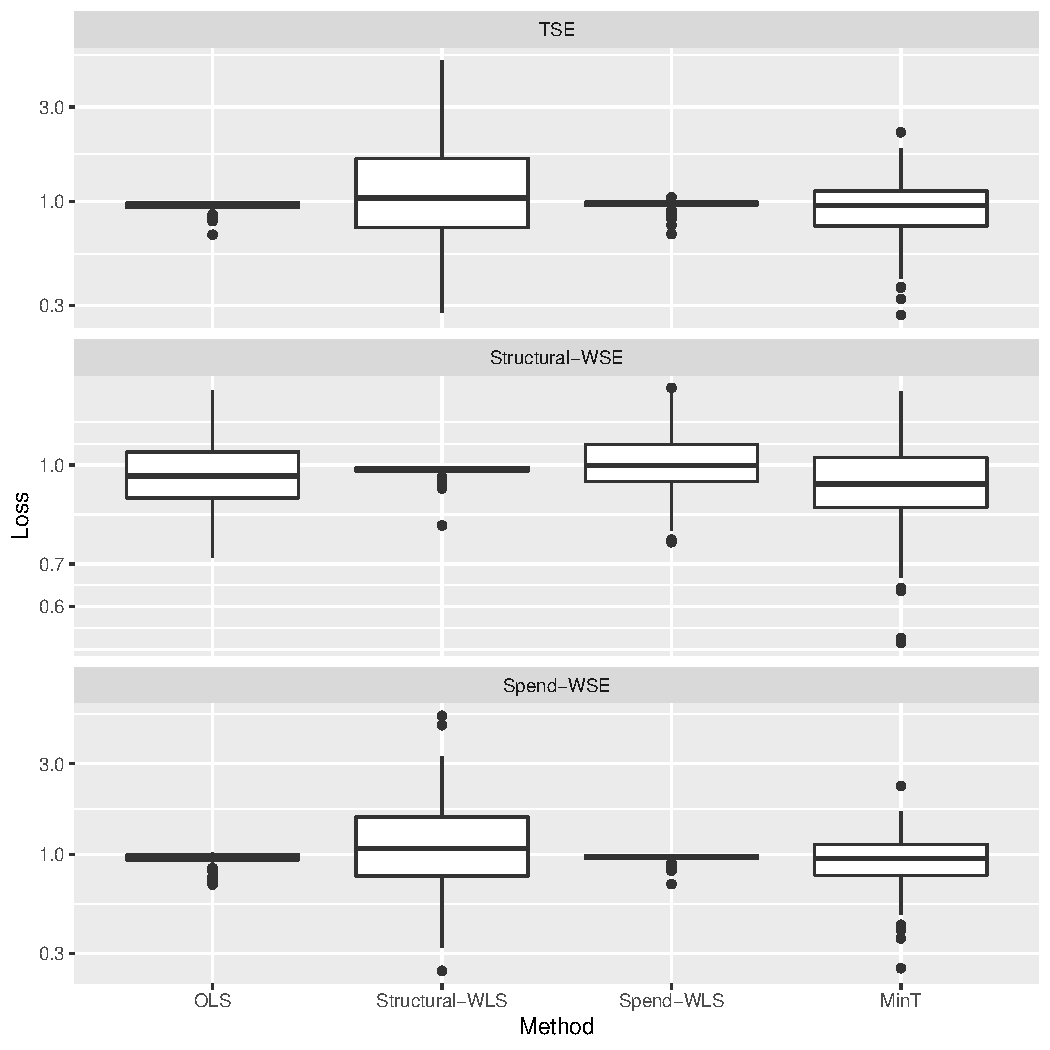
\includegraphics[width = \textwidth, height=14cm]{lossboxplots_2.pdf}
  		\caption{ Ratio of loss of reconciled forecast to loss of base forecast for $h = 1$. A value less than 1 indicates that the reconciled forecasts improve upon base forecasts.  A log scale is used for the y axis.}
  		\label{fig:BaseVSRecon_Fch2}
  	\end{figure}
    	\begin{figure}[!hbt]
  	\centering
  	\small
  	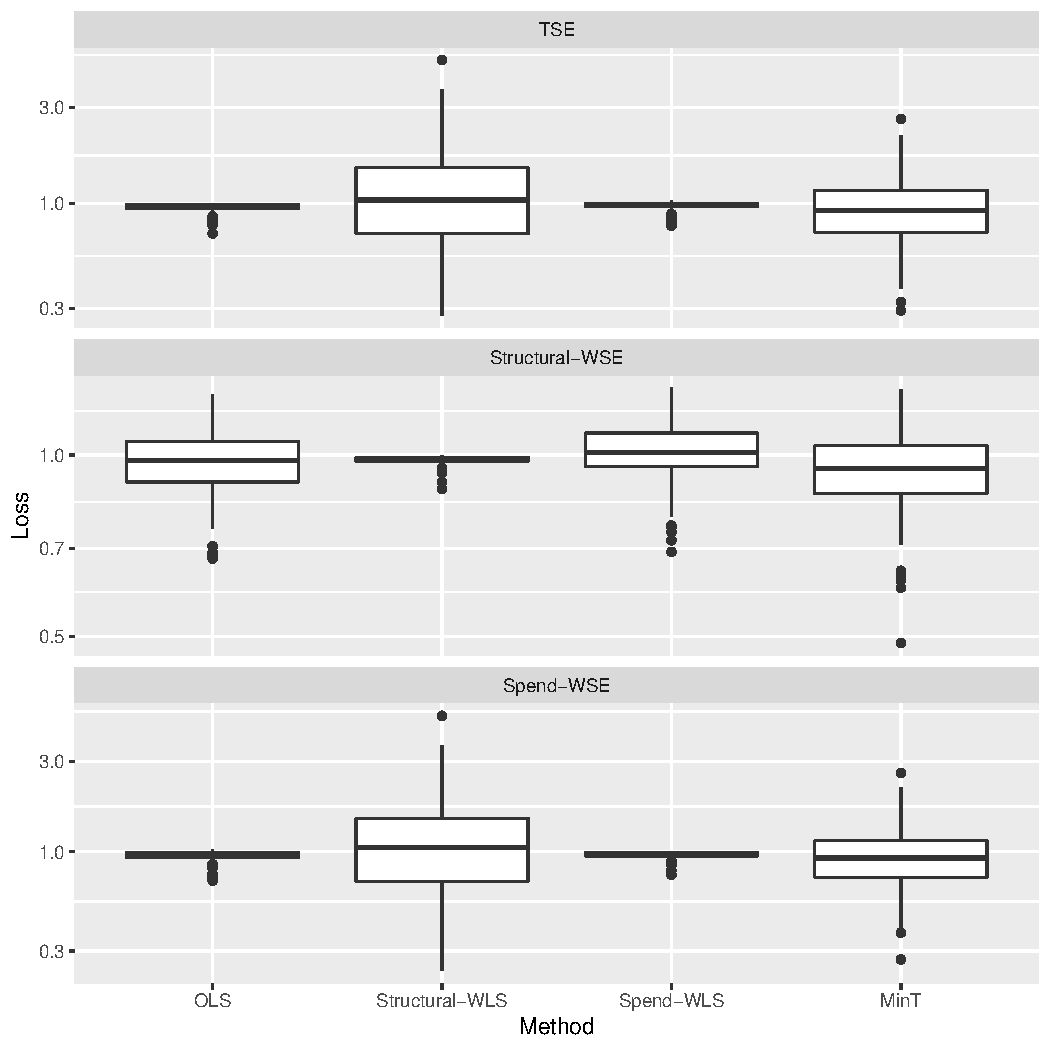
\includegraphics[width = \textwidth, height=14cm]{lossboxplots_3.pdf}
  	\caption{Ratio of loss of reconciled forecast to loss of base forecast for $h = 1$. A value less than 1 indicates that the reconciled forecasts improve upon base forecasts.  A log scale is used for the y axis.}
  	\label{fig:BaseVSRecon_Fch3}
  \end{figure}
  	\begin{figure}[!hbt]
	\centering
	\small
	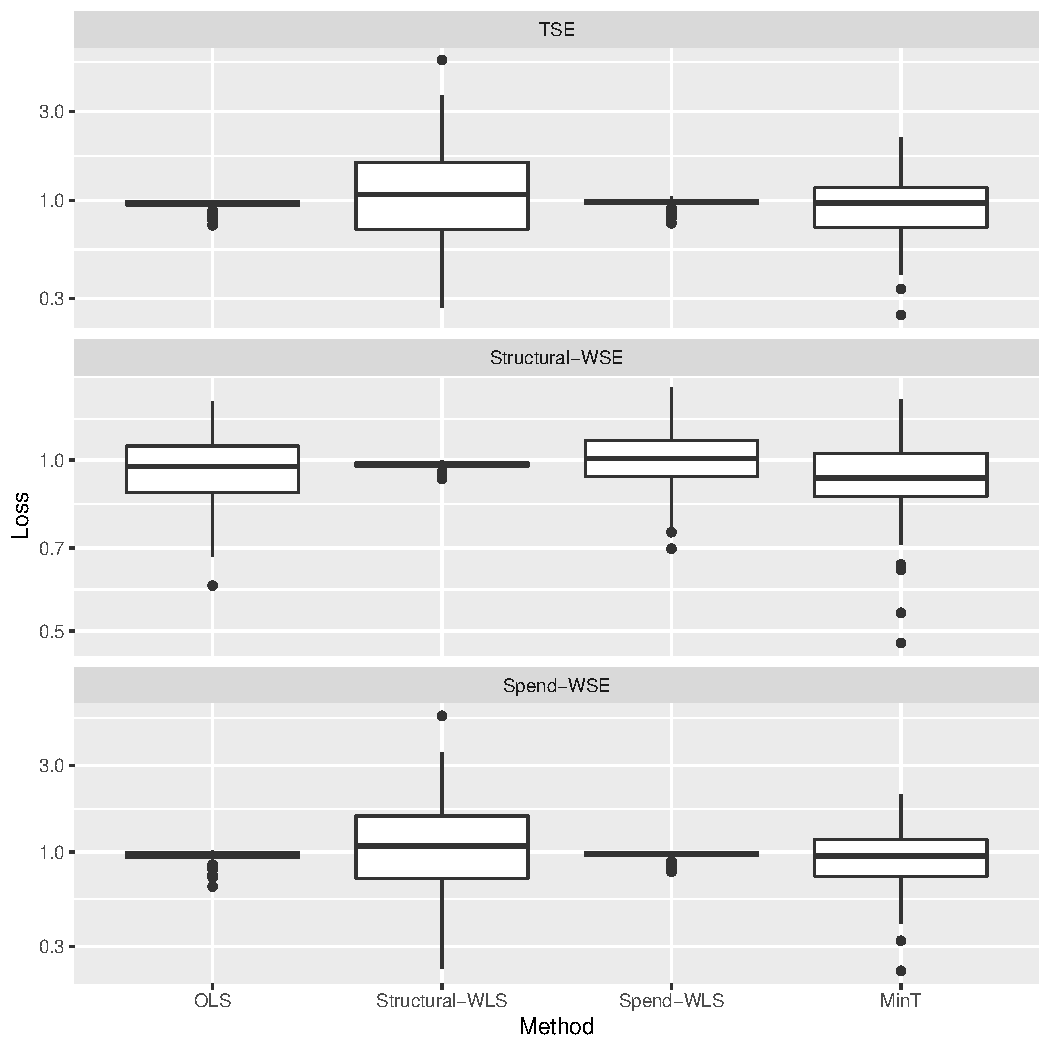
\includegraphics[width = \textwidth, height=14cm]{lossboxplots_4.pdf}
	\caption{Ratio of loss of reconciled forecast to loss of base forecast for $h = 1$. A value less than 1 indicates that the reconciled forecasts improve upon base forecasts.  A log scale is used for the y axis.}
	\label{fig:BaseVSRecon_Fch4}
\end{figure}
  	\begin{figure}[!hbt]
	\centering
	\small
	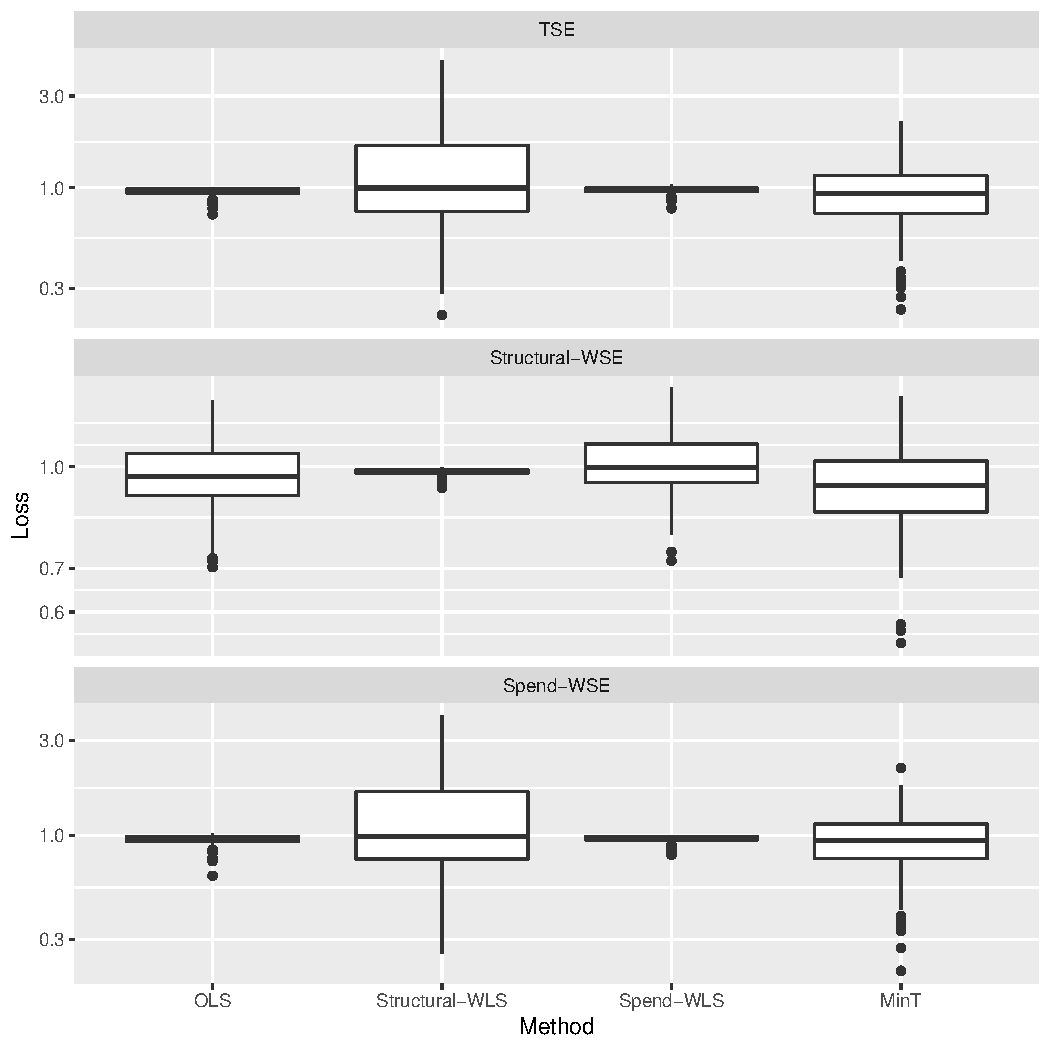
\includegraphics[width = \textwidth, height=14cm]{lossboxplots_5.pdf}
	\caption{Ratio of loss of reconciled forecast to loss of base forecast for $h = 1$. A value less than 1 indicates that the reconciled forecasts improve upon base forecasts.  A log scale is used for the y axis.}
	\label{fig:BaseVSRecon_Fch5}
\end{figure}
  	\begin{figure}[!hbt]
	\centering
	\small
	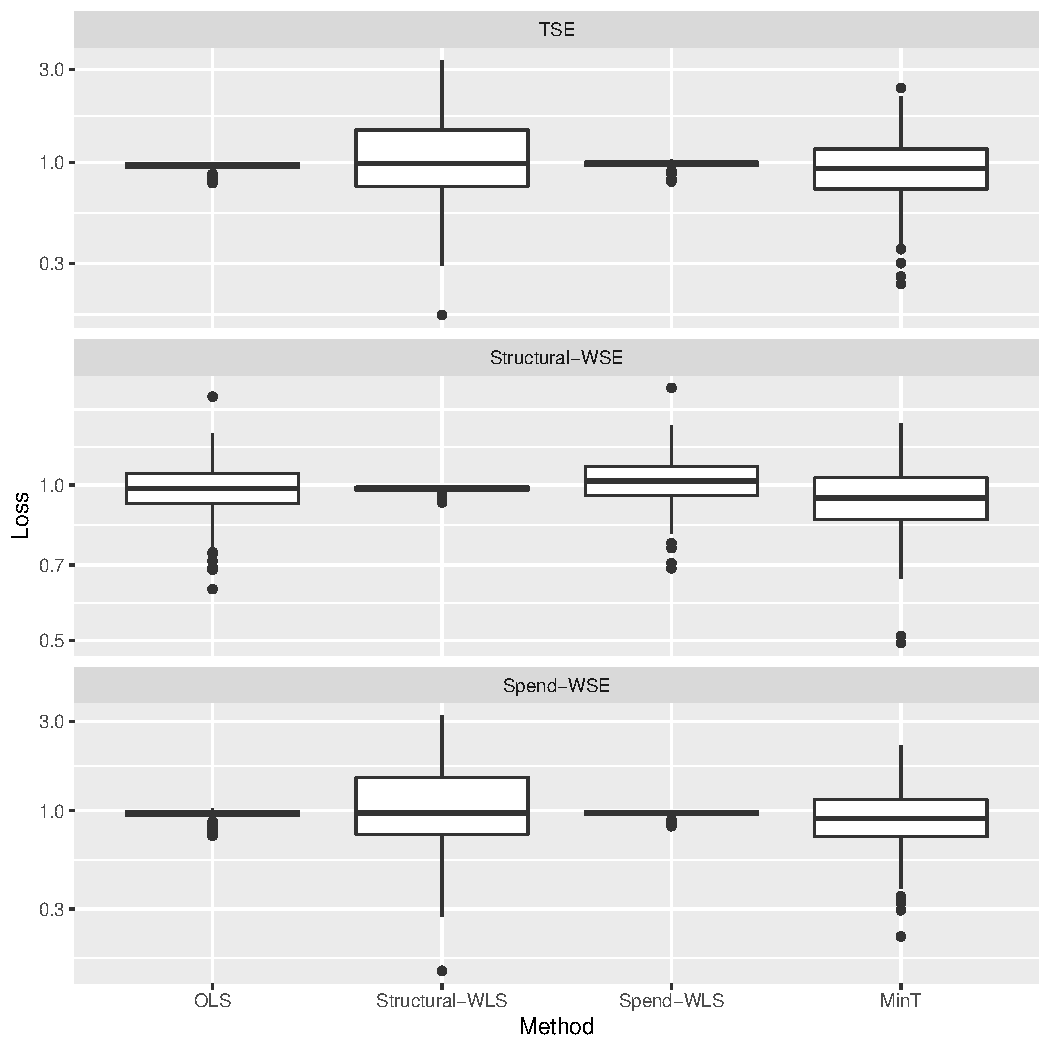
\includegraphics[width = \textwidth, height=14cm]{lossboxplots_6.pdf}
	\caption{ Ratio of loss of reconciled forecast to loss of base forecast for $h = 1$. A value less than 1 indicates that the reconciled forecasts improve upon base forecasts.  A log scale is used for the y axis.}
	\label{fig:BaseVSRecon_Fch6}
\end{figure}
  	
  	Tables ~\ref{tab:sec52h2} through to~\ref{tab:sec52h6} demonstrate Theorem 3.3; namely that MinT minimises expected loss irrespective of the choice of the weighting matrix.  For these results, an average loss is taken over all replications.  These averages are all expressed relative to base.  
  	
  	
  	\begin{table}[ht]
  		\centering
  		\begin{tabular}{lrrrrrr}
  			\hline
  			Loss Function & Base & Bottom-up & OLS & Structural-WLS & Spend-WLS & MinT \\ 
  			\hline
  			TSE & 1.00 & 1.27 & 0.97 & 1.17 & 0.98 & 0.97 \\ 
  			Structural WSE & 1.00 & 1.01 & 0.96 & 0.98 & 0.99 & 0.93 \\ 
  			Spend WSE & 1.00 & 1.25 & 0.97 & 1.16 & 0.98 & 0.96 \\ 
  			\hline
  		\end{tabular}
  		\caption{Means of different loss functions for 2-step ahead forecasts using different reconciliation methods in the tourism application.  All figures are reported relative to base forecasts.}
  		\label{tab:sec52h2} 
  	\end{table}
  	
  	\begin{table}[ht]
  		\centering
  		\begin{tabular}{lrrrrrr}
  			\hline
  			Loss Function & Base & Bottom-up & OLS & Structural-WLS & Spend-WLS & MinT \\ 
  			\hline
  			TSE & 1.00 & 1.25 & 0.97 & 1.16 & 0.98 & 0.97 \\ 
  			Structural WSE & 1.00 & 1.00 & 0.96 & 0.98 & 1.00 & 0.93 \\ 
  			Spend WSE & 1.00 & 1.23 & 0.97 & 1.15 & 0.98 & 0.96 \\ 
  			\hline
  		\end{tabular}
  		\caption{Means of different loss functions for 3-step ahead forecasts using different reconciliation methods in the tourism application.  All figures are reported relative to base forecasts.} 
  	\end{table}
  	
  	\begin{table}[ht]
  		\centering
  		\begin{tabular}{lrrrrrr}
  			\hline
  			Loss Function & Base & Bottom-up & OLS & Structural-WLS & Spend-WLS & MinT \\ 
  			\hline
  			TSE & 1.00 & 1.27 & 0.98 & 1.17 & 0.98 & 0.97 \\ 
  			Structural WSE & 1.00 & 1.01 & 0.96 & 0.98 & 0.99 & 0.92 \\ 
  			Spend WSE & 1.00 & 1.26 & 0.97 & 1.16 & 0.98 & 0.97 \\ 
  			\hline
  		\end{tabular}
  		\caption{Means of different loss functions for 4-step ahead forecasts using different reconciliation methods in the tourism application.  All figures are reported relative to base forecasts.} 
  	\end{table}
  
  \begin{table}[ht]
  	\centering
  	\begin{tabular}{lrrrrrr}
  		\hline
  		Loss Function & Base & Bottom-up & OLS & Structural-WLS & Spend-WLS & MinT \\ 
  		\hline
  		TSE & 1.00 & 1.28 & 0.98 & 1.18 & 0.98 & 0.97 \\ 
  		Structural WSE & 1.00 & 1.01 & 0.96 & 0.98 & 0.99 & 0.92 \\ 
  		Spend WSE & 1.00 & 1.26 & 0.97 & 1.17 & 0.98 & 0.96 \\ 
  		\hline
  	\end{tabular}
  	\caption{Means of different loss functions for 5-step ahead forecasts using different reconciliation methods in the tourism application.  All figures are reported relative to base forecasts.} 
  \end{table}

  \begin{table}[ht]
    \centering
	\begin{tabular}{lrrrrrr}
		\hline
		Loss Function & Base & Bottom-up & OLS & Structural-WLS & Spend-WLS & MinT \\ 
		\hline
		TSE & 1.00 & 1.21 & 0.98 & 1.13 & 0.99 & 0.97 \\ 
		Structural WSE & 1.00 & 1.00 & 0.97 & 0.98 & 1.00 & 0.93 \\ 
		Spend WSE & 1.00 & 1.20 & 0.98 & 1.12 & 0.98 & 0.97 \\ 
		\hline
	\end{tabular}
	\caption{Means of different loss functions for 6-step ahead forecasts using different reconciliation methods in the tourism application.  All figures are reported relative to base forecasts.}
	\label{tab:sec52h6} 
  \end{table}

  \section{Results for $h=2$ to $h=6$ for Section~5.3}
  
  George to include
   
\end{document}